% Options for packages loaded elsewhere
\PassOptionsToPackage{unicode}{hyperref}
\PassOptionsToPackage{hyphens}{url}
%
\documentclass[
  man,floatsintext]{apa6}
\usepackage{amsmath,amssymb}
\usepackage{lmodern}
\usepackage{iftex}
\ifPDFTeX
  \usepackage[T1]{fontenc}
  \usepackage[utf8]{inputenc}
  \usepackage{textcomp} % provide euro and other symbols
\else % if luatex or xetex
  \usepackage{unicode-math}
  \defaultfontfeatures{Scale=MatchLowercase}
  \defaultfontfeatures[\rmfamily]{Ligatures=TeX,Scale=1}
\fi
% Use upquote if available, for straight quotes in verbatim environments
\IfFileExists{upquote.sty}{\usepackage{upquote}}{}
\IfFileExists{microtype.sty}{% use microtype if available
  \usepackage[]{microtype}
  \UseMicrotypeSet[protrusion]{basicmath} % disable protrusion for tt fonts
}{}
\makeatletter
\@ifundefined{KOMAClassName}{% if non-KOMA class
  \IfFileExists{parskip.sty}{%
    \usepackage{parskip}
  }{% else
    \setlength{\parindent}{0pt}
    \setlength{\parskip}{6pt plus 2pt minus 1pt}}
}{% if KOMA class
  \KOMAoptions{parskip=half}}
\makeatother
\usepackage{xcolor}
\usepackage{color}
\usepackage{fancyvrb}
\newcommand{\VerbBar}{|}
\newcommand{\VERB}{\Verb[commandchars=\\\{\}]}
\DefineVerbatimEnvironment{Highlighting}{Verbatim}{commandchars=\\\{\}}
% Add ',fontsize=\small' for more characters per line
\usepackage{framed}
\definecolor{shadecolor}{RGB}{248,248,248}
\newenvironment{Shaded}{\begin{snugshade}}{\end{snugshade}}
\newcommand{\AlertTok}[1]{\textcolor[rgb]{0.94,0.16,0.16}{#1}}
\newcommand{\AnnotationTok}[1]{\textcolor[rgb]{0.56,0.35,0.01}{\textbf{\textit{#1}}}}
\newcommand{\AttributeTok}[1]{\textcolor[rgb]{0.77,0.63,0.00}{#1}}
\newcommand{\BaseNTok}[1]{\textcolor[rgb]{0.00,0.00,0.81}{#1}}
\newcommand{\BuiltInTok}[1]{#1}
\newcommand{\CharTok}[1]{\textcolor[rgb]{0.31,0.60,0.02}{#1}}
\newcommand{\CommentTok}[1]{\textcolor[rgb]{0.56,0.35,0.01}{\textit{#1}}}
\newcommand{\CommentVarTok}[1]{\textcolor[rgb]{0.56,0.35,0.01}{\textbf{\textit{#1}}}}
\newcommand{\ConstantTok}[1]{\textcolor[rgb]{0.00,0.00,0.00}{#1}}
\newcommand{\ControlFlowTok}[1]{\textcolor[rgb]{0.13,0.29,0.53}{\textbf{#1}}}
\newcommand{\DataTypeTok}[1]{\textcolor[rgb]{0.13,0.29,0.53}{#1}}
\newcommand{\DecValTok}[1]{\textcolor[rgb]{0.00,0.00,0.81}{#1}}
\newcommand{\DocumentationTok}[1]{\textcolor[rgb]{0.56,0.35,0.01}{\textbf{\textit{#1}}}}
\newcommand{\ErrorTok}[1]{\textcolor[rgb]{0.64,0.00,0.00}{\textbf{#1}}}
\newcommand{\ExtensionTok}[1]{#1}
\newcommand{\FloatTok}[1]{\textcolor[rgb]{0.00,0.00,0.81}{#1}}
\newcommand{\FunctionTok}[1]{\textcolor[rgb]{0.00,0.00,0.00}{#1}}
\newcommand{\ImportTok}[1]{#1}
\newcommand{\InformationTok}[1]{\textcolor[rgb]{0.56,0.35,0.01}{\textbf{\textit{#1}}}}
\newcommand{\KeywordTok}[1]{\textcolor[rgb]{0.13,0.29,0.53}{\textbf{#1}}}
\newcommand{\NormalTok}[1]{#1}
\newcommand{\OperatorTok}[1]{\textcolor[rgb]{0.81,0.36,0.00}{\textbf{#1}}}
\newcommand{\OtherTok}[1]{\textcolor[rgb]{0.56,0.35,0.01}{#1}}
\newcommand{\PreprocessorTok}[1]{\textcolor[rgb]{0.56,0.35,0.01}{\textit{#1}}}
\newcommand{\RegionMarkerTok}[1]{#1}
\newcommand{\SpecialCharTok}[1]{\textcolor[rgb]{0.00,0.00,0.00}{#1}}
\newcommand{\SpecialStringTok}[1]{\textcolor[rgb]{0.31,0.60,0.02}{#1}}
\newcommand{\StringTok}[1]{\textcolor[rgb]{0.31,0.60,0.02}{#1}}
\newcommand{\VariableTok}[1]{\textcolor[rgb]{0.00,0.00,0.00}{#1}}
\newcommand{\VerbatimStringTok}[1]{\textcolor[rgb]{0.31,0.60,0.02}{#1}}
\newcommand{\WarningTok}[1]{\textcolor[rgb]{0.56,0.35,0.01}{\textbf{\textit{#1}}}}
\usepackage{graphicx}
\makeatletter
\def\maxwidth{\ifdim\Gin@nat@width>\linewidth\linewidth\else\Gin@nat@width\fi}
\def\maxheight{\ifdim\Gin@nat@height>\textheight\textheight\else\Gin@nat@height\fi}
\makeatother
% Scale images if necessary, so that they will not overflow the page
% margins by default, and it is still possible to overwrite the defaults
% using explicit options in \includegraphics[width, height, ...]{}
\setkeys{Gin}{width=\maxwidth,height=\maxheight,keepaspectratio}
% Set default figure placement to htbp
\makeatletter
\def\fps@figure{htbp}
\makeatother
\setlength{\emergencystretch}{3em} % prevent overfull lines
\providecommand{\tightlist}{%
  \setlength{\itemsep}{0pt}\setlength{\parskip}{0pt}}
\setcounter{secnumdepth}{-\maxdimen} % remove section numbering
% Make \paragraph and \subparagraph free-standing
\ifx\paragraph\undefined\else
  \let\oldparagraph\paragraph
  \renewcommand{\paragraph}[1]{\oldparagraph{#1}\mbox{}}
\fi
\ifx\subparagraph\undefined\else
  \let\oldsubparagraph\subparagraph
  \renewcommand{\subparagraph}[1]{\oldsubparagraph{#1}\mbox{}}
\fi
\newlength{\cslhangindent}
\setlength{\cslhangindent}{1.5em}
\newlength{\csllabelwidth}
\setlength{\csllabelwidth}{3em}
\newlength{\cslentryspacingunit} % times entry-spacing
\setlength{\cslentryspacingunit}{\parskip}
\newenvironment{CSLReferences}[2] % #1 hanging-ident, #2 entry spacing
 {% don't indent paragraphs
  \setlength{\parindent}{0pt}
  % turn on hanging indent if param 1 is 1
  \ifodd #1
  \let\oldpar\par
  \def\par{\hangindent=\cslhangindent\oldpar}
  \fi
  % set entry spacing
  \setlength{\parskip}{#2\cslentryspacingunit}
 }%
 {}
\usepackage{calc}
\newcommand{\CSLBlock}[1]{#1\hfill\break}
\newcommand{\CSLLeftMargin}[1]{\parbox[t]{\csllabelwidth}{#1}}
\newcommand{\CSLRightInline}[1]{\parbox[t]{\linewidth - \csllabelwidth}{#1}\break}
\newcommand{\CSLIndent}[1]{\hspace{\cslhangindent}#1}
\ifLuaTeX
\usepackage[bidi=basic]{babel}
\else
\usepackage[bidi=default]{babel}
\fi
\babelprovide[main,import]{english}
% get rid of language-specific shorthands (see #6817):
\let\LanguageShortHands\languageshorthands
\def\languageshorthands#1{}
% Manuscript styling
\usepackage{upgreek}
\captionsetup{font=singlespacing,justification=justified}

% Table formatting
\usepackage{longtable}
\usepackage{lscape}
% \usepackage[counterclockwise]{rotating}   % Landscape page setup for large tables
\usepackage{multirow}		% Table styling
\usepackage{tabularx}		% Control Column width
\usepackage[flushleft]{threeparttable}	% Allows for three part tables with a specified notes section
\usepackage{threeparttablex}            % Lets threeparttable work with longtable

% Create new environments so endfloat can handle them
% \newenvironment{ltable}
%   {\begin{landscape}\centering\begin{threeparttable}}
%   {\end{threeparttable}\end{landscape}}
\newenvironment{lltable}{\begin{landscape}\centering\begin{ThreePartTable}}{\end{ThreePartTable}\end{landscape}}

% Enables adjusting longtable caption width to table width
% Solution found at http://golatex.de/longtable-mit-caption-so-breit-wie-die-tabelle-t15767.html
\makeatletter
\newcommand\LastLTentrywidth{1em}
\newlength\longtablewidth
\setlength{\longtablewidth}{1in}
\newcommand{\getlongtablewidth}{\begingroup \ifcsname LT@\roman{LT@tables}\endcsname \global\longtablewidth=0pt \renewcommand{\LT@entry}[2]{\global\advance\longtablewidth by ##2\relax\gdef\LastLTentrywidth{##2}}\@nameuse{LT@\roman{LT@tables}} \fi \endgroup}

% \setlength{\parindent}{0.5in}
% \setlength{\parskip}{0pt plus 0pt minus 0pt}

% Overwrite redefinition of paragraph and subparagraph by the default LaTeX template
% See https://github.com/crsh/papaja/issues/292
\makeatletter
\renewcommand{\paragraph}{\@startsection{paragraph}{4}{\parindent}%
  {0\baselineskip \@plus 0.2ex \@minus 0.2ex}%
  {-1em}%
  {\normalfont\normalsize\bfseries\itshape\typesectitle}}

\renewcommand{\subparagraph}[1]{\@startsection{subparagraph}{5}{1em}%
  {0\baselineskip \@plus 0.2ex \@minus 0.2ex}%
  {-\z@\relax}%
  {\normalfont\normalsize\itshape\hspace{\parindent}{#1}\textit{\addperi}}{\relax}}
\makeatother

% \usepackage{etoolbox}
\makeatletter
\patchcmd{\HyOrg@maketitle}
  {\section{\normalfont\normalsize\abstractname}}
  {\section*{\normalfont\normalsize\abstractname}}
  {}{\typeout{Failed to patch abstract.}}
\patchcmd{\HyOrg@maketitle}
  {\section{\protect\normalfont{\@title}}}
  {\section*{\protect\normalfont{\@title}}}
  {}{\typeout{Failed to patch title.}}
\makeatother

\usepackage{xpatch}
\makeatletter
\xapptocmd\appendix
  {\xapptocmd\section
    {\addcontentsline{toc}{section}{\appendixname\ifoneappendix\else~\theappendix\fi\\: #1}}
    {}{\InnerPatchFailed}%
  }
{}{\PatchFailed}
\keywords{keywords\newline\indent Word count: X}
\usepackage{csquotes}
\ifLuaTeX
  \usepackage{selnolig}  % disable illegal ligatures
\fi
\IfFileExists{bookmark.sty}{\usepackage{bookmark}}{\usepackage{hyperref}}
\IfFileExists{xurl.sty}{\usepackage{xurl}}{} % add URL line breaks if available
\urlstyle{same} % disable monospaced font for URLs
\hypersetup{
  pdftitle={EDLD 654 Final Project: Fiction Transportation Modeling Proof of Concept},
  pdfauthor={Eliott Doyle1},
  pdflang={en-EN},
  pdfkeywords={keywords},
  hidelinks,
  pdfcreator={LaTeX via pandoc}}

\title{EDLD 654 Final Project: Fiction Transportation Modeling Proof of Concept}
\author{Eliott Doyle\textsuperscript{1}}
\date{}


\shorttitle{EDLD 654 Final}

\affiliation{\vspace{0.5cm}\textsuperscript{1} University of Oregon}

\begin{document}
\maketitle

The GitHub repository for this project can be found at \url{https://github.com/ekgekd/EDLD654final}

\hypertarget{research-problem}{%
\subsection{Research Problem}\label{research-problem}}

Last year I collected data for my master's project, in which participants in three experimental conditions wrote short stories, letters, or journal entries and responded to some surveys and demographic questions. Subsequently, several research assistants coded these writing samples for \emph{transportation}: the extent to which the reader (i.e., the coder) feels that they were immersed or swept up in the text.

Transportation is one of the main operationalizations of audience involvement when reading a text; the degree to which someone experiences transportation while reading generally predicts how much they are emotionally affected by the text, how much they identify with the characters, and how much they are persuaded by the text's message (Green, Brock, \& Kaufman, 2004).

I am interested in how author features contribute to their ability to write a text that is transporting to readers. My research more broadly focuses on empathic accuracy, or, how well people are able to understand what another person is feeling during interactions. The manner in which the target (or, person being perceived, who the perceiver is attempting to empathize with) expresses themselves affects how well the perceived is able to pick up on their thoughts and feelings, and features like how invested the target is in what they are communicating, experience communicating with others, and emotional expressivity can influence how easy their communication is to parse for a perceiver. While transportation does not directly tie to empathic accuracy, it is related, in that it is a measure of how compelled the perceiver is by the target's words.

Most past research on transportation has focused on the features of the perceiver/audience rather than of the author. I am interested in investigating author features. Identifying characteristics of authors that make them better at writing texts that produce high transportation in others will help illuminate what makes communication more effective. Being able to model the transportation scores of texts based on the text and characteristics of the author will be informative in my understanding of what aspects of authors' experience while writing leads to more effective writing that has an impact on readers/perceivers.

\hypertarget{description-of-the-data}{%
\subsection{Description of the Data}\label{description-of-the-data}}

264 University of Oregon undergraduates participated in this study and produced data that was usable for the current analyses. The sample size was adequate for the ANOVA and linear regression analyses I conducted for hypothesis testing, but because it is relatively small for machine learning purposes, I will be considering this a proof of concept for future applications similar to this, rather than a definitive model for predicting transportation.

\emph{Predicted variable: Transportation.} Seven research assistants coded the writing samples for transportation on a Likert scale ranging from 1 (no transportation) to 5 (very high transportation). The mean scores from all seven research assistants make up the transportation variable.

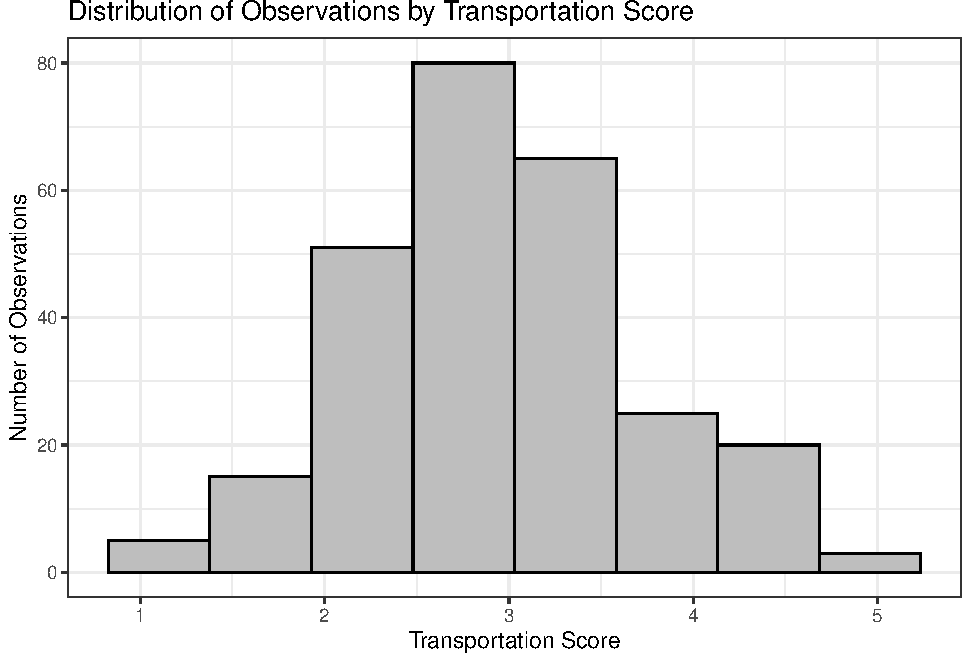
\includegraphics{Final_Eliott_files/figure-latex/unnamed-chunk-1-1.pdf}

\emph{Writing samples.} The writing samples were personal in nature and so are confidential. I have gotten the embeddings from the samples without the samples themselves, and saved those for the purposes of this project.

\emph{Writing experience.} Authors reported how much experience they have with writing fiction and journaling, within the past year and prior to the past year when they participated in the study. These were four separate questions that here will be treated as one measure with mean scores for the four questions representing writing experience. 1 indicates no writing experience; 3 indicates frequent and long-time writing experience in different forms. Mean writing experience was 1.610 with standard deviation 0.434, indicating that authors generally had some writing experience but not a lot, with a lot of variability.

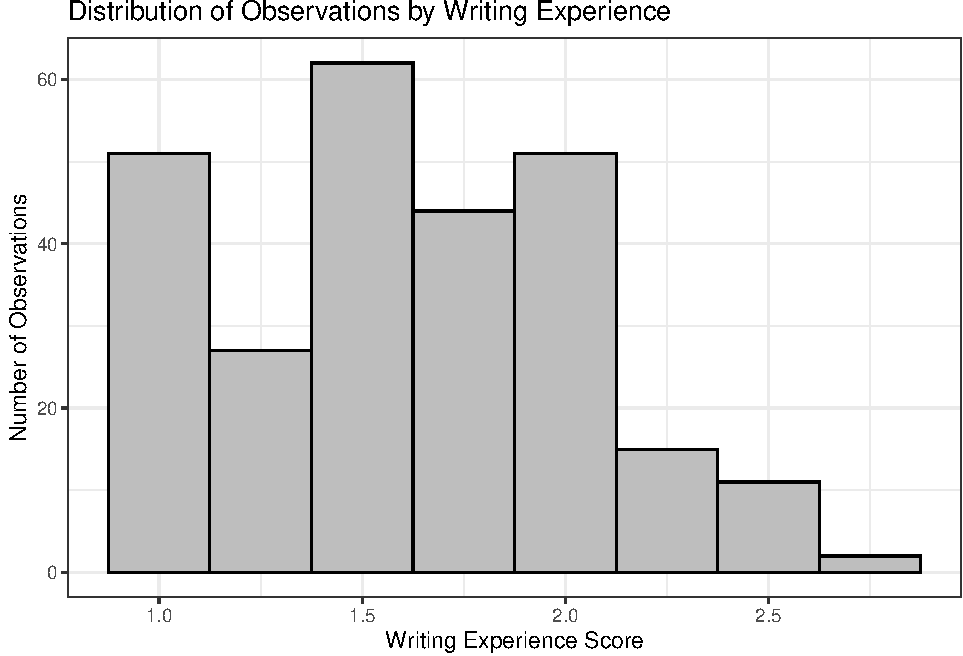
\includegraphics{Final_Eliott_files/figure-latex/unnamed-chunk-3-1.pdf}

\emph{Interpersonal Reactivity Index (IRI).} The IRI (Davis, 1983) is a popular measure of trait empathy. The authors of the writing samples completed this survey, so this is a measure of author trait empathy, not perceiver empathy. The IRI comprises 28 questions; the mean score for each other is reported with 1 being very low empathy and 5 being very high empathy. Mean IRI score was 3.468, with SD = 0.444. The distribution of responses was normal.

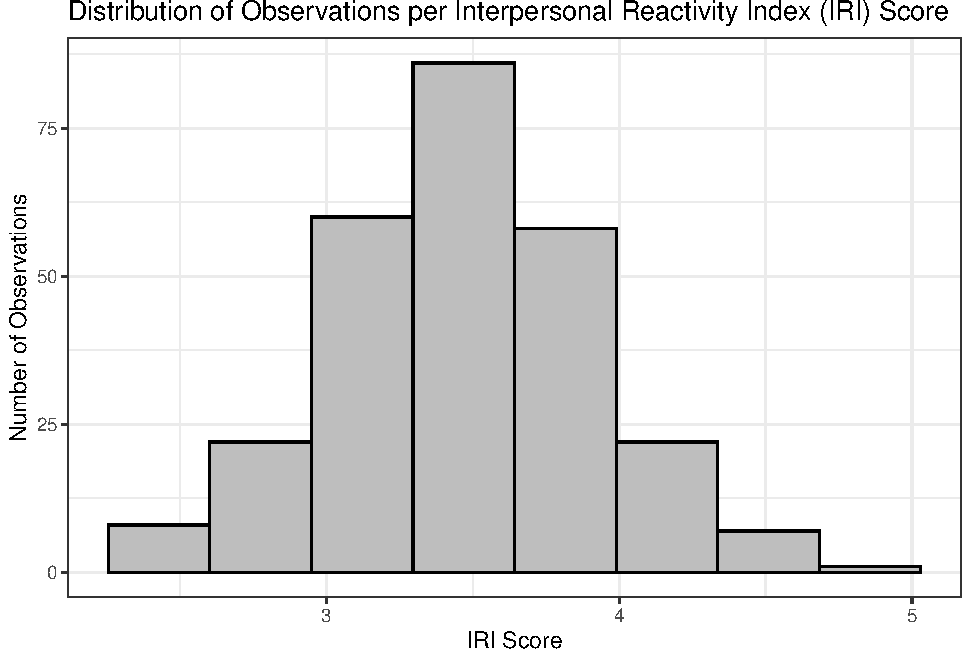
\includegraphics{Final_Eliott_files/figure-latex/unnamed-chunk-5-1.pdf}

\emph{Character liking.} Authors rated how much they liked the characters they were writing about on a measure of liking comprising 9 questions. The mean score for each author is reported with 1 being strong dislike for the character and 5 being strong liking for the character. Mean character liking was 3.566 with SD = 0.771. Liking was fairly high presumably because authors were instructed to choose their favorite fictional character.

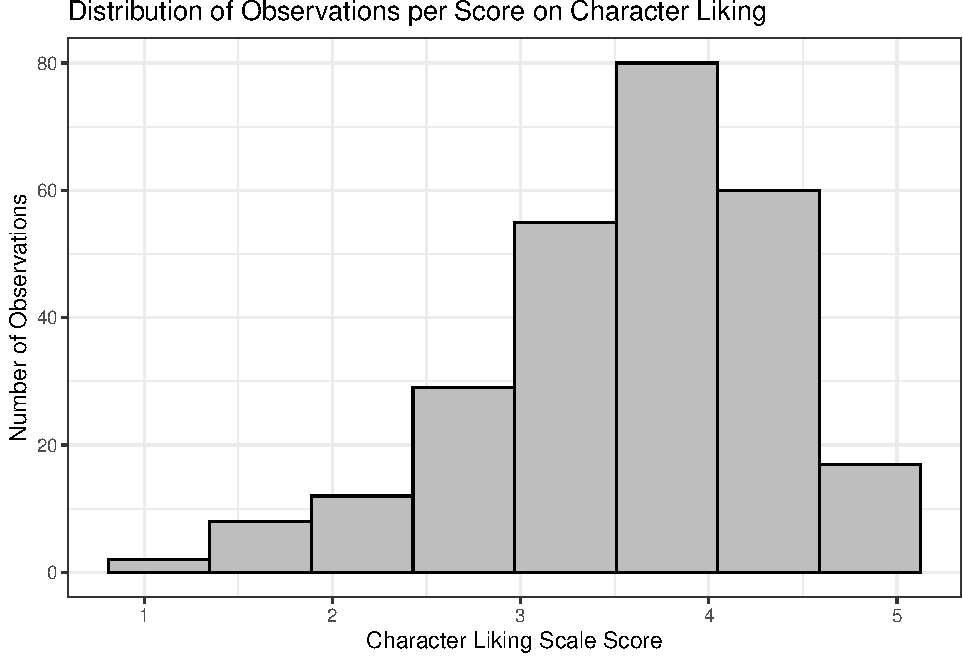
\includegraphics{Final_Eliott_files/figure-latex/unnamed-chunk-7-1.pdf}

\emph{Missingness.}

These data have already been cleaned, so there are not many missing values. No variable is missing more than a few data points, so I have not dropped any of my variables from the analyses.

\hypertarget{description-of-the-models}{%
\section{Description of the Models}\label{description-of-the-models}}

Describe each model fit, why the given
model was selected, which hyperparameters to be optimized and how,
assumptions of the model, and a high-level (think broad audience) description of
what the model is doing and why it is appropriate (even as an initial starting
point). Also, discuss how you plan to evaluate model performance.

\hypertarget{model-1-linear-regression.}{%
\paragraph{Model 1: Linear Regression.}\label{model-1-linear-regression.}}

I chose to start with a linear regression model without penalty because I am trying to predict a continuous variable using predictor variables, and I want to know which of those predictor variables are the most helpful in predicting transportation scores. This model looks at all the predictor variables I have, and tells us how much of the variance in transportation scores is predicted by the linear relationship between the predictor variables and transportation. I want to start with this model because it is relatively straightforward, but it might have issues with modeling patterns that aren't there because I have more predictor variables than I have samples. There are no hyperparameters to tune for this model.

\hypertarget{model-2-ridge-regression.}{%
\paragraph{Model 2: Ridge Regression.}\label{model-2-ridge-regression.}}

My next model is regression with ridge penalty. I will need to tune the lambda value for this model. It might be a good idea to implement a penalty because I have a lot of predictor variables, some of which I expect to be correlated with each other, and because I do not have as many samples as I have predictor variables. Using ridge regression will reduce sampling variation to help avoid modeling the noise of the data, and hopefully only capture signal. In other words, I have a lot of predictors and not a lot of samples, so there will be a tendency for a linear regression without penalty to make predictions of patterns that aren't there. Doing a ridge regression will put some constraints on the model to cut out meaningless patterns that might show up in the plain linear regression model.

\hypertarget{model-3-bagged-trees.}{%
\paragraph{Model 3: Bagged Trees.}\label{model-3-bagged-trees.}}

Finally, I will model the data using bagged trees. This will provide a non-linear model of the data, in case a linear approach is not the best way to look at the relationships between variables in my data. This model is based on decision trees: in a decision tree analysis, individual continuous variables are split at some optimal point, below which the analysis is conducted differently from the observations above the cutoff. This can be done for any number of variables, any number of times. It is difficult to predict which variables and which cut points will be best (hyperparameters that would need to be tuned, in a decision tree analysis), so it is best to do a lot of decision trees with cuts at different places to determine which is best. I opted to use bagged trees instead of random forests because random forests randomizes rows as well as columns and I have a very limited number of rows. For this analysis, the hyperparameter that will need to be tuned is the number of trees.

\hypertarget{evaluation-of-model-performance.}{%
\paragraph{Evaluation of Model Performance.}\label{evaluation-of-model-performance.}}

I will compare the root mean squared error (RMSE), mean absolute error (MAE), and R-square of the test data. I will be looking for low values for the error terms (RMSE and MAE) and high values of R-square to determine the best model for my data.

\hypertarget{model-fit}{%
\section{Model Fit}\label{model-fit}}

\hypertarget{linear-regression-model.}{%
\paragraph{Linear Regression Model.}\label{linear-regression-model.}}

\begin{verbatim}
## glmnet 
## 
## 198 samples
## 772 predictors
## 
## Recipe steps: normalize, impute_mean 
## Resampling: Cross-Validated (10 fold) 
## Summary of sample sizes: 178, 178, 178, 179, 178, 178, ... 
## Resampling results:
## 
##   RMSE      Rsquared   MAE      
##   0.480031  0.6164308  0.3721775
## 
## Tuning parameter 'alpha' was held constant at a value of 0
## Tuning
##  parameter 'lambda' was held constant at a value of 0
\end{verbatim}

\begin{verbatim}
##   alpha lambda     RMSE  Rsquared       MAE     RMSESD RsquaredSD      MAESD
## 1     0      0 0.480031 0.6164308 0.3721775 0.07266484  0.1184717 0.06785649
\end{verbatim}

\begin{verbatim}
## [1] 0.4526108
\end{verbatim}

\begin{verbatim}
## [1] 0.4005285
\end{verbatim}

\begin{verbatim}
## [1] 0.5219195
\end{verbatim}

\hypertarget{ridge-regression-model.}{%
\paragraph{Ridge Regression Model.}\label{ridge-regression-model.}}

Below is a plot of RMSE for different values of lambda. RMSE is flat until lambda is greater than 4, at which point RMSE goes up rapidly.

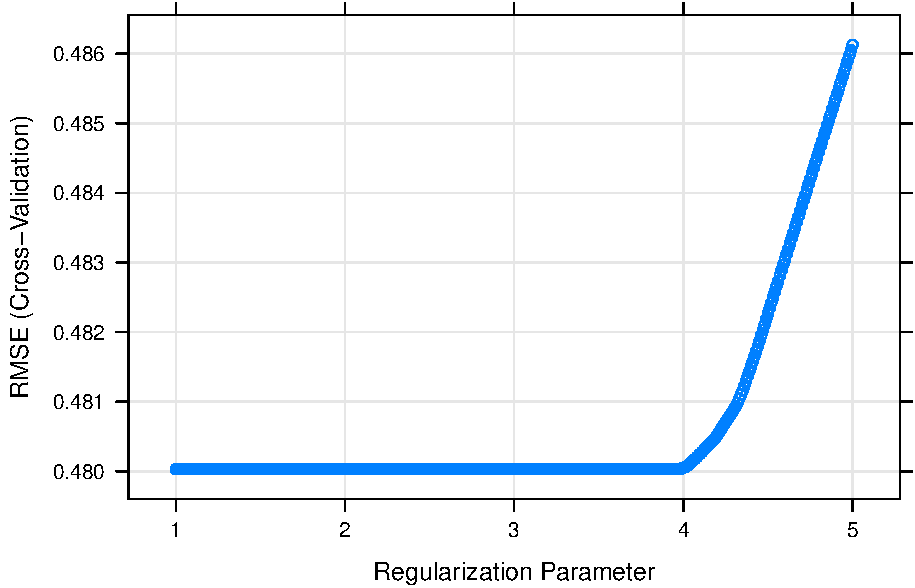
\includegraphics{Final_Eliott_files/figure-latex/unnamed-chunk-20-1.pdf}

The best lambda value for this model is 3.97, so I will be proceeding with that. The results for the model using that lambda value are:

\begin{verbatim}
##     alpha lambda     RMSE  Rsquared       MAE     RMSESD RsquaredSD      MAESD
## 298     0   3.97 0.480031 0.6164308 0.3721775 0.07266484  0.1184717 0.06785649
\end{verbatim}

Below are the importance evaluations of each of the predictors in this model:

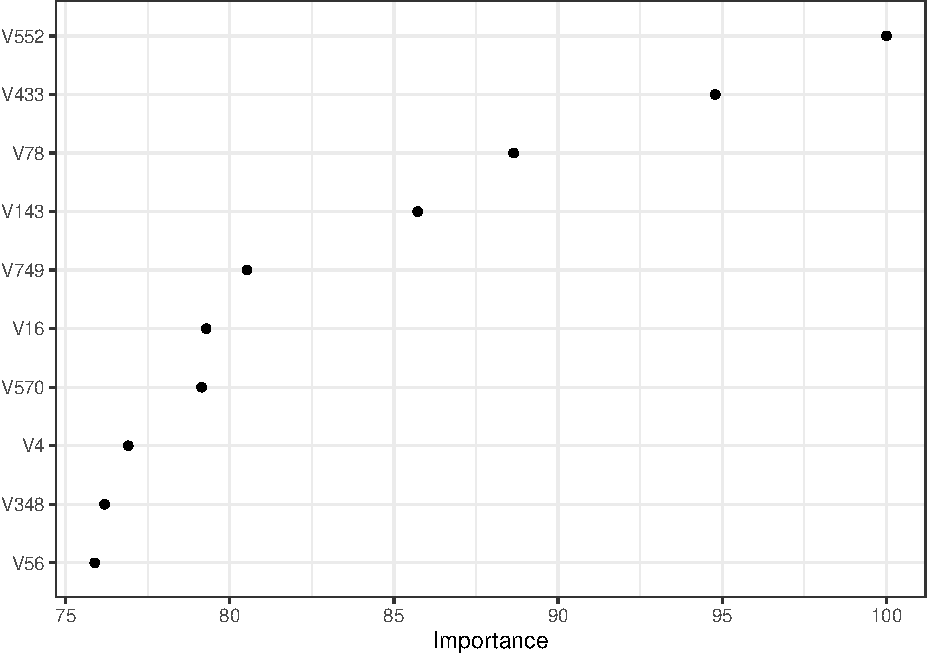
\includegraphics{Final_Eliott_files/figure-latex/unnamed-chunk-23-1.pdf}
The top ten most important predictors in this model are all encodings of the text data

\hypertarget{bagged-trees.}{%
\paragraph{Bagged Trees.}\label{bagged-trees.}}

\begin{verbatim}
##   mtry splitrule min.node.size      RMSE  Rsquared       MAE    RMSESD
## 1  771  variance             2 0.5815234 0.4051429 0.4583493 0.1088807
##   RsquaredSD      MAESD
## 1  0.1418285 0.08519205
\end{verbatim}

Below is a plot of RMSEs for the model using different numbers of trees. The minimum RMSE comes from a model using 160 trees, so I will proceed with that.

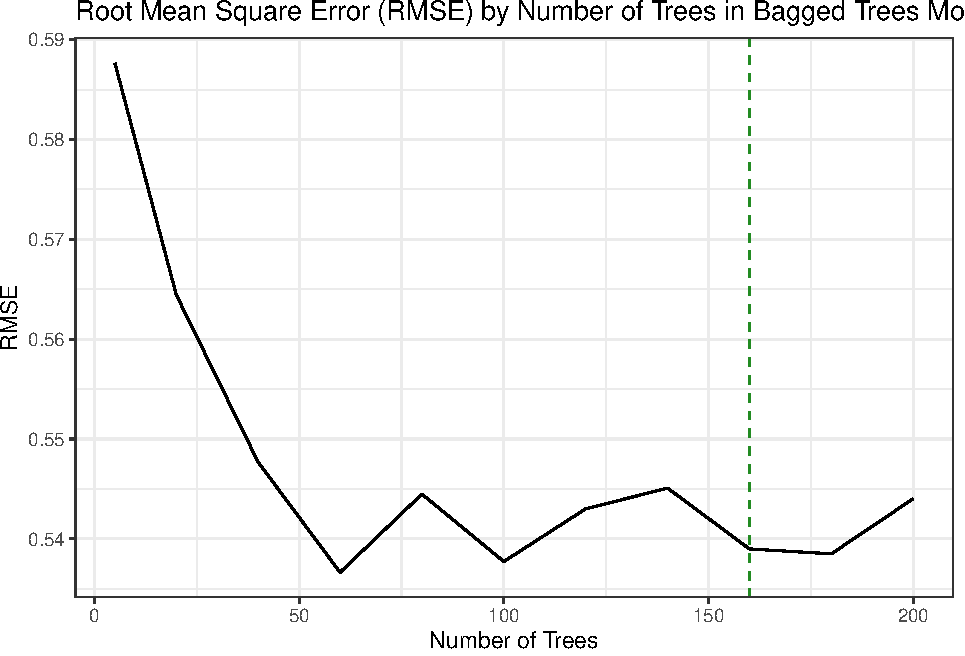
\includegraphics{Final_Eliott_files/figure-latex/unnamed-chunk-31-1.pdf}

\begin{Shaded}
\begin{Highlighting}[]
\NormalTok{nbags[}\FunctionTok{which.min}\NormalTok{(rmses)]}
\end{Highlighting}
\end{Shaded}

\begin{verbatim}
## [1] 60
\end{verbatim}

\hypertarget{model-comparison}{%
\section{Model Comparison}\label{model-comparison}}

\begin{verbatim}
##                   R-sq       MAE      RMSE
## Linear       0.4526108 0.4005285 0.5219195
## Ridge        0.4526108 0.4005285 0.5219195
## Bagged Trees 0.1406842 0.5370130 0.6835069
\end{verbatim}

The bagged trees model yields a lower R-square and higher MAE and higher RMSE than either regression model. I would therefore choose not to use bagged trees for this analysis.

All terms are identical for linear regression without penalty and for linear regression with ridge penalty. The RMSE was the same in the ridge regression model for all lambda values up to the optimal cutoff point, and non-penalized linear regression uses a lambda value of 0, which is why these models aren't different. This tells us that overfitting is not an issue for linear regression in these data. I would favor linear regression over ridge regression because it's simpler to run, but functionally it makes no real difference.

\hypertarget{discussion}{%
\section{Discussion}\label{discussion}}

The regression models were the best for predicting the transportation score of the writing samples provided by the participants in my study. Linear regression without penalty and with ridge penalty were equally predictive; neither was excellent, but both were better at predicting transportation than the bagged trees model.

Some of the text encodings were the most important in predicting transportation score: the text samples themselves seem to do a better job of predicting how transporting readers will find the writing than features of the writer. This is not necessarily unexpected, as transportation scores came from research assistants reading the writing samples (with no knowledge of the participants' backgrounds or personalities). This is interesting because it suggests that people can write stories that are transporting to readers more or less regardless of their personal qualities --- at least, in the case of these very short stories. This also indicates that I should look into other features of the writing itself that can be operationalized that underlies transportation scores --- in other words, what do the encodings mean, and could we code for/name them so as to develop a better model with or without these encodings? It is somewhat inconvenient not to know what exactly the encodings mean, since it is hard to come to any real conclusions about what features of the text lead to transportation that are psychologically meaningful. It is helpful to have a model that can predict transportation based on text, but it does not mean very much, and might not be very satisfying if I were to write it up in a report for a psychological journal. However, the small sample size makes it so that using this model would not be a good idea.

Overall, the conclusion I get from this is that the participant features included in this model (empathy scale scores, writing experience, and liking of the character they were writing about) probably are not the most important features to look at when determining how transporting their writing will be. In the future, it might be useful to build a model like this that uses text encodings that could predict how transporting text samples are so that human coders would not have to code thousands upon thousands of new text samples, and then to use the predictions from the model instead of transportation scores from human coders as the transportation variable in larger-scale studies --- if we were not reliant on human coders to determine transportation because we had a model that could assign transportation scores reasonably well, then we could use the model's predictions as a variable, and then use participant self-report to determine the relationship between empathy score or writing experience or other variables. So, going forward, if I planned to do large-scale studies trying to explain what features of a writer lead them to write transporting stories, it would be helpful to collect a lot of text samples and have human coders rate them on transportation in order to build a model in a pilot study, and then use the model's scores instead of human coders' transportation score in the actual study.

\newpage

\textbf{REFERENCES}

\hypertarget{refs}{}
\begin{CSLReferences}{1}{0}
\leavevmode\vadjust pre{\hypertarget{ref-IRI1983}{}}%
Davis, M. H. (1983). Measuring individual differences in empathy: Evidence for a multidimensional approach. \emph{Journal of Personality and Social Psychology}, \emph{44}, 113.

\leavevmode\vadjust pre{\hypertarget{ref-Green2004}{}}%
Green, M. C., Brock, T. C., \& Kaufman, G. F. (2004). Understanding media enjoyment: The role of transportation into narrative worlds. \emph{Communication Theory}, \emph{14}, 311--327.

\end{CSLReferences}


\end{document}
